\section{Modelul Bohr}

Ideea corectă a modelului Rutherford de existență a unui nucleu atomic în care
este concentrată aproape toată masa și toată sarcina pozitivă a atomului a fost
preluată în modelele atomice propuse ulterior.

În conceptul lui Bohr, atomul este un sistem solar în miniatură, cu forțe
electrice în loc de forțe gravitaționale. Nucleul încărcat pozitiv joacă rolul
soarelui, iar electronii se mișcă în jurul lui sub acțiunea forțelor electrice
de atracție.

Acest model atomic se bazează pe \emph{postulatele lui Bohr}.

În fizica clasică, energia unui sistem poate varia în mod continuu.

Având o masă mai mică decât a atomilor, electronii nu vor pierde energie la o
ciocnire, ci vor fi \emph{împrăștiați elastic}. Însă în urma unei ciocniri
inelastice cu un atom, electronul va pierde energie, iar viteza lui va scădea.
Energia pierdută va fi transferată atomului ciocnit, care trece într-o
\emph{stare excitată}. Se constată, pe cale experimentală, că atomul poate
primi energie numai în anumite valori bine determinate.
\emph{Atomul poate avea numai anumite stări (discrete) de energie}.

\emph{Cuanta} de radiație este unitatea structurală de bază a câmpurilor ce
poate fi emisă sau absorbită de un sistem fizic (molecular, atomic, nuclear
etc.). De exemplu, fotonul pentru câmpul electromagnetic. Energia unei cuante
de radiație se mai numește \emph{cuantă de energie}.

\emph{Cuantificarea} este procedeul mecanicii cuantice prin care se impune ca
mărimile fizice ce caracterizează sistemul de particule să ia doar valori
discrete. De exemplu, energia, impulsul, momentul cinetic etc.

S-a constatat că intensitatea și frecvența radiației emise cresc odată cu
energia de excitare, raportul energie-frecvență fiind constanta lui Planck
(numită și \emph{cuantă de acțiune}):
\[ \frac{E}{\nu} = h = 6,626075 \cdot 10^{-34} ~ \mathrm{J \cdot s} \]

Se poate scrie că energia radiațiilor emise de atomii care se dezexcită este
proporțională cu frecvența:
\[ E = h\nu \]

În conceperea modelului cuantificat, au fost emise cele două postulate ale lui
Bohr:
\begin{enumerate}[label=\Roman*.]
    \item Atomii și sistemele atomice se pot găsi timp îndelungat numai în
        stări bine determinate, numite stări staționare, în care nu emit și nu
        absorb energie. \\
        Energia sistemului în aceste stări este cuantificată, adică ia valori
        ce alcătuiesc un șir discontinuu: \( E_1, E_2, ..., E_n \).
    \item Atomii emit sau absorb radiație electromagnetică doar la trecerea
        dintr-o stare staționară $m$, caracterizată de energia $E_m$, în altă
        stare staționară $n$, caracterizată de energia $E_n$. \\
        Frecvența radiației emise sau absorbite într-o astfel de tranziție este
        dată de relația:
        \[ h\nu_{mn} = E_m - E_n \]
        Acest postulat explică spectrele de linii ale radiațiilor emise de
        atomii de hidrogen.
\end{enumerate}

\subsection{%
    Cuantificarea distanțelor electronului față de nucleu%
    \texorpdfstring{ ($r_n$)}{}, a vitezelor lui pe orbita
    circulară\texorpdfstring{ ($v_n$)}{}, a impulsului%
    \texorpdfstring{ ($p_n$)}{}, și a energiei totale%
    \texorpdfstring{ ($E_n$)}{}
}

Aceste mărimi pot fi obținute considerând că forța coulombiană este o forță de
natură centripetă:
\begin{equation}
    \frac{e^2}{4\pi\varepsilon_0 r^2} = \frac{mv^2}{r}
    \label{eq:2}
\end{equation}
și că electronului i se poate asocia o undă cu lungimea de undă
\( \lambda_B = \frac{h}{p} \).

Pot exista numai acele orbite ale electronului în atom pentru care este
satisfăcută condiția existenței undelor de Broglie staționare. Pentru aceasta,
lungimea orbitei circulare trebuie să cuprindă un număr întreg de lungimi de
undă, adică exact \emph{condiția de cuantificare a momentului cinetic al
mișcării electronului pe o orbită staționară}:
\[ 2\pi r = n\lambda_B = \frac{nh}{mv} \]
\begin{center}
    sau
\end{center}
\begin{equation}
    mvr = n\frac{h}{2\pi} = n\overline{h}, ~ n \in \mathbb{N}^*
    \label{eq:3}
\end{equation}
unde $\overline{h}$ se numește constanta Planck redusă (sau constanta Dirac).

\begin{wrapfigure}{l}{0.4\textwidth}
    \centering
    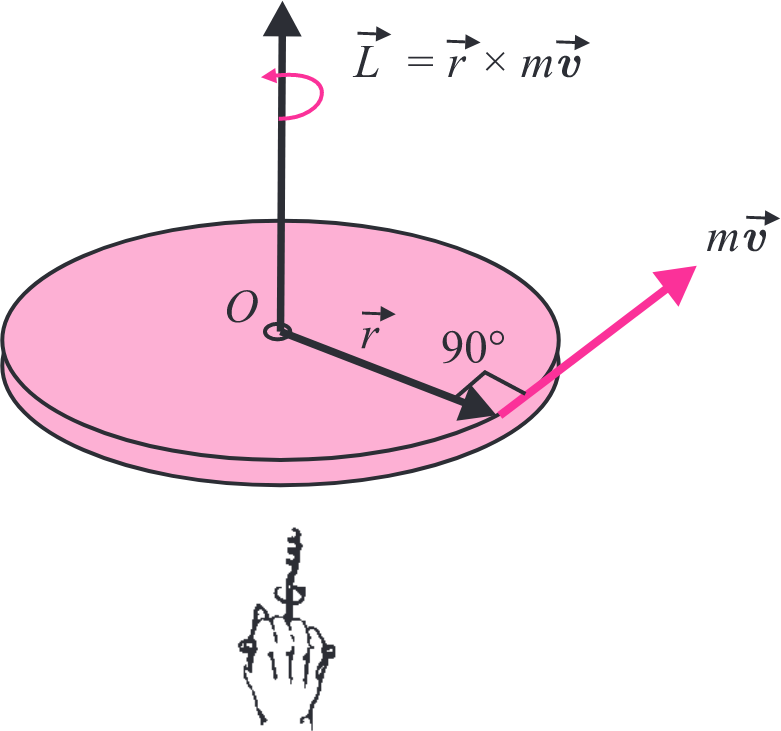
\includegraphics[width=0.35\textwidth]{fig/moment_cinetic}
    \caption{Momentul cinetic al punctului material în mișcarea circulară}
\end{wrapfigure}

\emph{Momentul cinetic} (sau \emph{moment al impulsului}) $\vec{L}$ este
analogul impulsului în mișcarea de rotație. Este definit ca produsul vectorial
dintre vectorul de poziție $\vec{r}$ al originii vectorului impuls, față de
centrul de rotație, și impulsul punctului material $\vec{p} = m\vec{v}$:
\[ \vec{L} = \vec{r} \times \vec{p} = \vec{r} \times m\vec{v} \]

Momentul cinetic este un vector cu modulul \( L = rp\sin(\vec{r}, m\vec{v}) \).
În mișcarea circulară, \( \vec{r} \perp m\vec{v} \), deci $L = rmv$. Se măsoară
în SI în kg \cdot\ m$^2$s$^{-1}$ = J \cdot s.

\clearpage

Postulatele lui Bohr nu decurg din niciun principiu al fizicii clasice, ci se
bazează doar pe fizica cuantică. Conform condiției de cuantificare a lui Bohr,
electronul se poate mișca în jurul nucleului doar pe acele orbite pentru care
$L$ este un multiplu al lui $\overline{h}$.

Din relațiile \eqref{eq:2} și \eqref{eq:3} pot fi deduse expresiile
cuantificate ale $r_n$, $v_n$, $p_n$, $E_n$:
\begin{align*}
    \frac{e^2}{4\pi\varepsilon_0 r^2} = \frac{mv^2}{r}
    &\Rightarrow v^2 = \frac{e^2}{4\pi\varepsilon_0 rm}
    \\
    rmv = n\frac{h}{2\pi} &\Rightarrow v^2 = \frac{n^2 h^2}{4\pi^2 m^2 r^2}
    \Rightarrow \boxed{v_n = \frac{nh}{2\pi mr_n}}
\end{align*}

Din aceste două exprimări ale $v^2$ rezultă
\( \frac{e^2}{4\pi\varepsilon_0 rm} = \frac{n^2 h^2}{4\pi^2 m^2 r^2} \), de
unde se obține:
\[
    \boxed{r_n = \frac{\varepsilon_0 h^2}{\pi me^2} n^2}
    \Rightarrow \boxed{v_n = \frac{e^2}{2\varepsilon_0 h} \frac{1}{n}}
\]
\[
    p_n = mv^n \Rightarrow
    \boxed{p_n = \frac{me^2}{2\varepsilon_0h} \frac{1}{n}}
\]

Din \eqref{eq:1} se obține:
\begin{equation}
    E_n = -\frac{e^2}{8\pi\varepsilon_0 r_n}
    \Rightarrow \boxed{E_n = -\frac{me^4}{8\varepsilon_0^2 h^2} \frac{1}{n^2}}
    \label{eq:4}
\end{equation}

Aplicăm expresiile deduse atomului de hidrogen $^1_1$H.
Pentru $n = 1$, raza primei orbite Bohr este:
\begin{equation}
    r_1 = \frac{\varepsilon_0 h^2}{\pi m e^2}, ~\text{iar}~ r_n = r_1n^2
    \label{eq:5}
\end{equation}
Orbitele neradiante permise au deci razele $r_1$, $4r_1$, $9r_1$ etc.

Știind
\begin{align*}
    \varepsilon_0 &= \SI{8,85d-12}{\coulomb\tothe{2}\per\newton\per\metre\tothe{2}}
    \hspace{0.75cm}
    &h &= \SI{6,62d-34}{\joule\cdot\second}
    \\
    m &= \SI{9,11d-31}{\kilogram}
    \hspace{0.75cm}
    &e &=\SI{1,60d-19}{\coulomb}
\end{align*}
se obține \( r_1 = \SI{0,53d-10}{\metre} \), valoare aflată în concordanță cu
diametrele atomice estimate prin alte metode.

Conform \eqref{eq:5}, distanța dintre două orbite consecutive crește odată cu
îndepărtarea de nucleu.

Orice sistem fizic tinde spre starea echilibru stabil, care corespunde energiei
cele mai joase. Energia sistemului nucleu-electron fiind negativă, starea
energetică cea mai joasă se atinge când această energie are valoarea absolută
cea mai mare, deci pentru $n = 1$.

Această stare, de energie minimă, se numește \emph{stare fundamentală} sau
\emph{normală}.

În cazul atomului de hidrogen, din relația \eqref{eq:4} rezultă:
\[ E_1 = -\frac{me^4}{8h^2\varepsilon_0^2} = \SI{-13,6}{\electronvolt} \]

\begin{wrapfigure}{l}{0.45\textwidth}
    \centering
    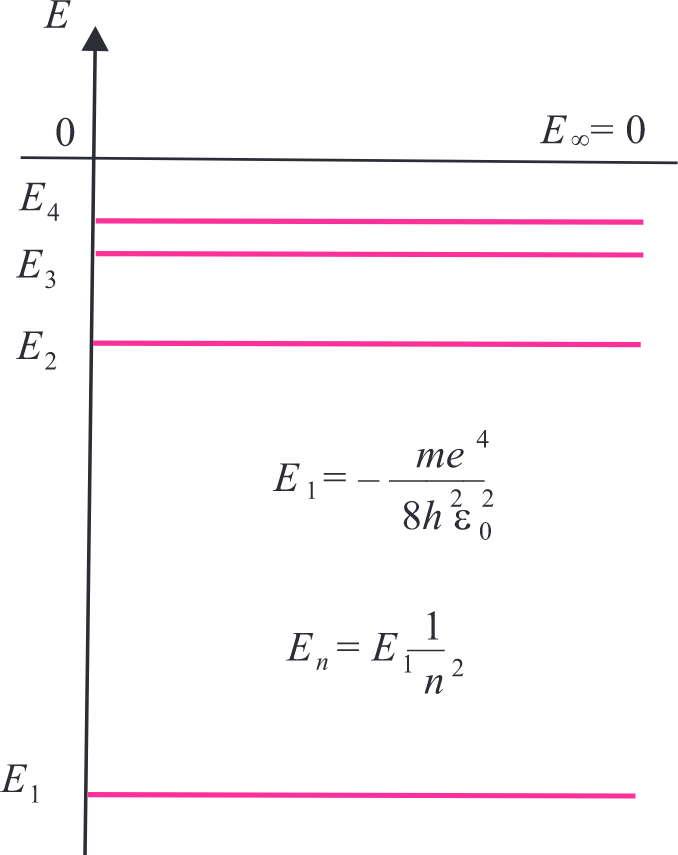
\includegraphics[width=0.4\textwidth]{fig/niveluri_energie_hidrogen}
    \caption{Nivelurile de energie ale atomului de hidrogen}
\end{wrapfigure}

În fig. 7, liniile orizontale indică \emph{nivelurile de energie} (valorile
energiei totale).

Originea se află în $E = 0$, pentru numere cuantice foarte mari, când
electronul este depărtat de nucleu și pierde legătura cu acesta (ionizare).

Deasupra $E = 0$ pot fi reprezentate valorile pozitive ale energiei, ce
corespund mișcării libere a electronului și care nu sunt cuantificate, fiind
posibilă orice valoare. \emph{Stările legate} ale electronului în atom sunt
exprimate prin energiile negative, reprezentate sub $E = 0$.

Se observă că nivelurile cuantificate se strâng spre 0.
\[ E_n = \frac{E_1}{n^2} \]

Relațiile deduse sunt aplicabile atomului de hidrogen și atomilor hidrogenoizi
(cu un singur electron): He$^+$ (o dată ionizat), Li$^{++}$ (de două ori
ionizat), Be$^{+++}$ (de trei ori ionizat) etc.

În general, pentru atomii hidrogenoizi, unde $Z$ este numărul atomic:
\[
    E_n = -\frac{mZ^2e^4}{8h^2\varepsilon_0^2}
    = -13,6 \cdot \frac{Z^2}{n^2} ~ \si{\electronvolt}
\]

\subsection{Seriile spectrale ale hidrogenului și ale atomilor hidrogenoizi}

Electronul poate trece din starea fundamentală într-o stare excitată prin
absorbția unui foton. Această stare excitată nu este stabilă.

Un atom se dezexcită în \SI{d-8}{\second}, energia înmagazinată fiind radiată
sub formă de energie a unei unde electromagnetice de frecvență bine
determinată, acoperind întregul domeniu spectral, de la infraroșu la
ultraviolet.

Energia fotonului emis sau absorbit la trecerea de la o stare staționară la
alta este dată de postulatul al II-lea al lui Bohr.

Urmează studiul spectrelor de emisie -- trecerea electronului dintr-o stare
excitată într-o stare de energie mai joasă, la emiterea unui foton de energie
$h\nu$ (prin dezexcitare).

Ne vom referi la spectrul de emisie al atomului de hidrogen (H), care este un
spectru de linii.

Fie $n-i$ numărul cuantic al unei stări excitate oarecare, și $n_f$ numărul
cuantic al stării de energie mai joase, pe care se întoarce electronul după
emisie.

Energia inițială este:
\[ E_i = -\frac{me^4}{8\varepsilon_0 h^2} \frac{1}{n_i^2} \]

Energia finală este:
\[ E_f = -\frac{me^4}{8\varepsilon_0 h^2} \frac{1}{n_f^2} \]

Energia fotonului emis, $h\nu$, va fi egală cu:
\[
    E_i - E_f = h\nu
    = -\frac{me^4}{8\varepsilon_0 h^2} \frac{1}{n_i^2}
    + \frac{me^4}{8\varepsilon_0 h^2} \frac{1}{n_f^2}
\]

Frecvența liniei emise, $\nu$, va fi:
\[
    \nu = \frac{me^4}{8\varepsilon_0 h^2}
    \left(\frac{1}{n_f^2} - \frac{1}{n_i^2}\right)
\]

Introducem notația pentru \emph{numărul de undă} $\tilde{\nu}$ -- numărul de
lungimi de undă cuprinse în intervalul unitate:
\[ \tilde{\nu} = \frac{\nu}{c} = \frac{1}{cT} = \frac{1}{\lambda} \]

Atunci:
\[
    \tilde{\nu} = \frac{me^4}{8\varepsilon_0 h^2}
    \left(\frac{1}{n_f^2} - \frac{1}{n_i^2}\right)
\]

Mărimea $\frac{me^4}{8\varepsilon_0 h^2}$ este \emph{constanta lui Rydberg},
având valoarea $R = \SI{1,097373d7}{\per\meter}$.

Astfel, energia cuantificată a electronului pe un nivel energetic al atomului
poate fi exprimată ca:
\[ \boxed{E_n = -\frac{Rch}{n^2}} \]

Grupul de linii spectrale cu același $n_f$ formează o \emph{serie spectrală}.

Pentru $n_i \rightarrow \infty$, numărul de undă este maxim, cu valoarea
$\frac{R}{n^2}$, numită limita seriei.

\emph{Inversele lungimilor de undă ale liniilor spectrale emise de atomul de
hidrogen} sunt date de ecuația:
\[ \tilde{\nu} = R \left(\frac{1}{n_f^2} - \frac{1}{n_i^2}\right) \]
iar pentru \emph{atomii hidrogenoizi}, cu sarcina $Ze$ și un singur electron,
de ecuația:
\[ \tilde{\nu} = RZ^2 \left(\frac{1}{n_f^2} - \frac{1}{n_i^2}\right) \]

\clearpage

\begin{wrapfigure}{r}{0.45\textwidth}
    \centering
    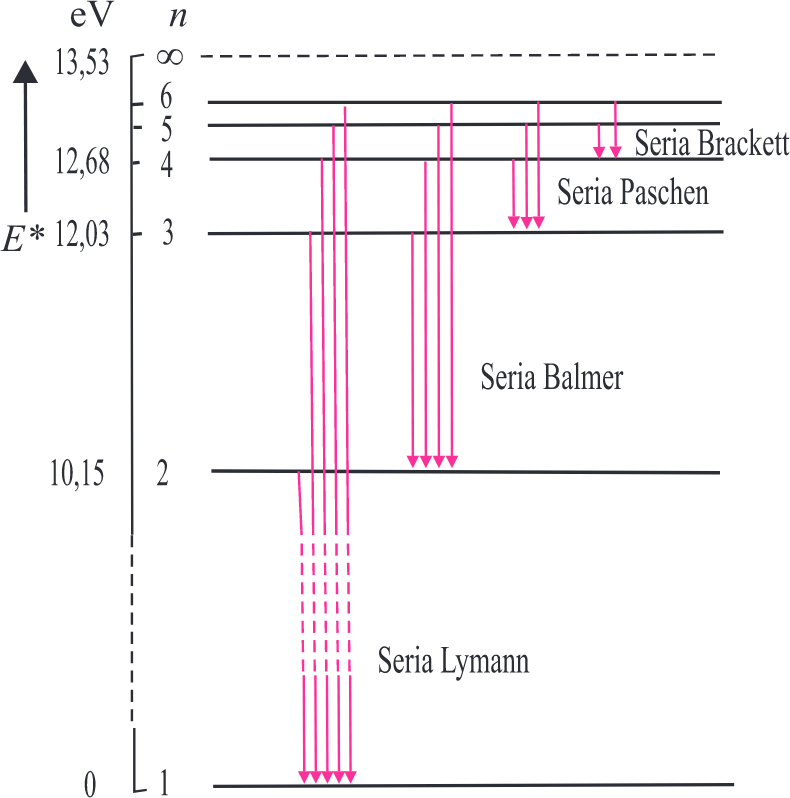
\includegraphics[width=0.4\textwidth]{fig/tranzitii_electron}
    \caption{Tranzițiile electronului în modelul Bohr al atomului de hidrogen}
\end{wrapfigure}

Cu mult înainte ca Bohr să elaboreze modelul atomic al hidrogenului, studiind
liniile din vizibil ale atomului, Balmer a observat că lungimile de undă ale
liniilor spectrale emise respectă anumite regularități.

Rydberg a rearanjat \emph{relația empirică a lui Balmer}, pentru calculul
lungimilor de undă:
\[ \tilde{\nu} = \frac{1}{\lambda} = R\left(\frac{1}{2^2} - \frac{1}{n^2\right}) \]

S-a obținut empiric aceeași valoare a lui $R$ ca în modelul atomic al lui Bohr.

Seriile spectrale ale hidrogenului sunt redate în tabelul următor.

Tranzițiile sunt ilustrate în fig. 8, și pot fi realizate direct sau în trepte.
Numărul tranzițiilor posibile este egal cu $C_n^2 = \frac{(n-1)n}{2}$.

\begin{center}
    \renewcommand{\arraystretch}{1.5}
    \begin{tabular}{|c|c|c|c|c|}
        \hline
        \textbf{Denumirea seriei spectrale} & \boldmath$n_f$ & \boldmath$n_i$ &
        \textbf{Domeniul spectral} & \textbf{Limita seriei} \\
        \hline
        Lyman & 1 & 2, 3, ... & ultraviolet & $R$ \\
        \hline
        Balmer & 2 & 3, 4, ... & vizibil & $R/4$ \\
        \hline
        Paschen & 3 & 4, 5, ... & infraroșu & $R/9$ \\
        \hline
        Brackett & 4 & 5, 6, ... & infraroșu & $R/16$ \\
        \hline
        Pfund & 5 & 6, 7, ... & infraroșu îndepărtat & $R/25$ \\
        \hline
    \end{tabular}
\end{center}

\subsection*{Aplicații ale spectroscopiei}

Spectroscopia este o metodă comodă, precisă, și rapidă în analiza chimică, cu
ajutorul acesteia fiind descoperite elementele cesiu, taliu, indiu, și galiu.

Sursele moderne de iluminare, precum tuburile cu descărcare rapidă în vapori de
sodiu sau mercur, sau lămpile fluorescente, au fost inventate pe baza studiilor
spectroscopice.

Ceasul atomic este instrumentul de măsurare a timpului cel mai precis, utilizat
de exemplu la GPS. O secundă este egală cu 9192631770 perioade asociate
tranziției între două niveluri energetice ale cesiului 133.

Cele mai importante utilizări ale spectroscopiei au avut loc în astronomie, în
studiul temperaturii, compoziției, și deplasării astrelor.
